\section{Casos de uso}

\subsection*{Encargado de compras}
\begin{enumerate}
	\item Consultar precios disponibles para un producto,  
	por número de parte, nombre o descripción del producto,
	considerando distintos proveedores,
	para optar por aquel que ofrezca mejores condiciones,
	contando con la información para negociar el mejor precio de compra posible.
	\item Conocer los precios de la competencia,
	para tener un parámetro con el cual comparar precios de compra,
	y descubrir oportunidades en productos con márgenes relativamente mayores.
	\item Seguir el stock disponible,
	de manera que sea posible preveer necesidades de corto y mediano plazo.
\end{enumerate}

\subsection*{Encargado de ventas}
\begin{enumerate}
	\item Conocer los precios de la competencia,
	para tener un parámetro con el cual establecer el precio de venta propio.
	\item Conocer precio de compra,
	para tener un parámetro de la base para obtener rentabilidad
	y fijar precios que permitan encontrar un equilibrio entre competitividad y margen de ganancia.
	\item Fijar precios de venta a consumidor final,
	que serán utilizados por el personal de ventas.
\end{enumerate}

\subsection*{Personal de ventas}
\begin{enumerate}
	\item Consultar precios de los productos para informar al consumidor final que lo requiera.
	\item Confirmar disponibilidad de stock de producto al consumidor final que lo requiera.
	\item Emitir factura electrónica,
	con la autorización correspondiente de ARCA,
	restando del conteo de stock el producto vendido.
\end{enumerate}

\pagebreak 

\section{Diagrama de casos de uso}

\begin{figure}[h!]
	\vspace{20pt}
	\centering
	\vspace{15pt}
	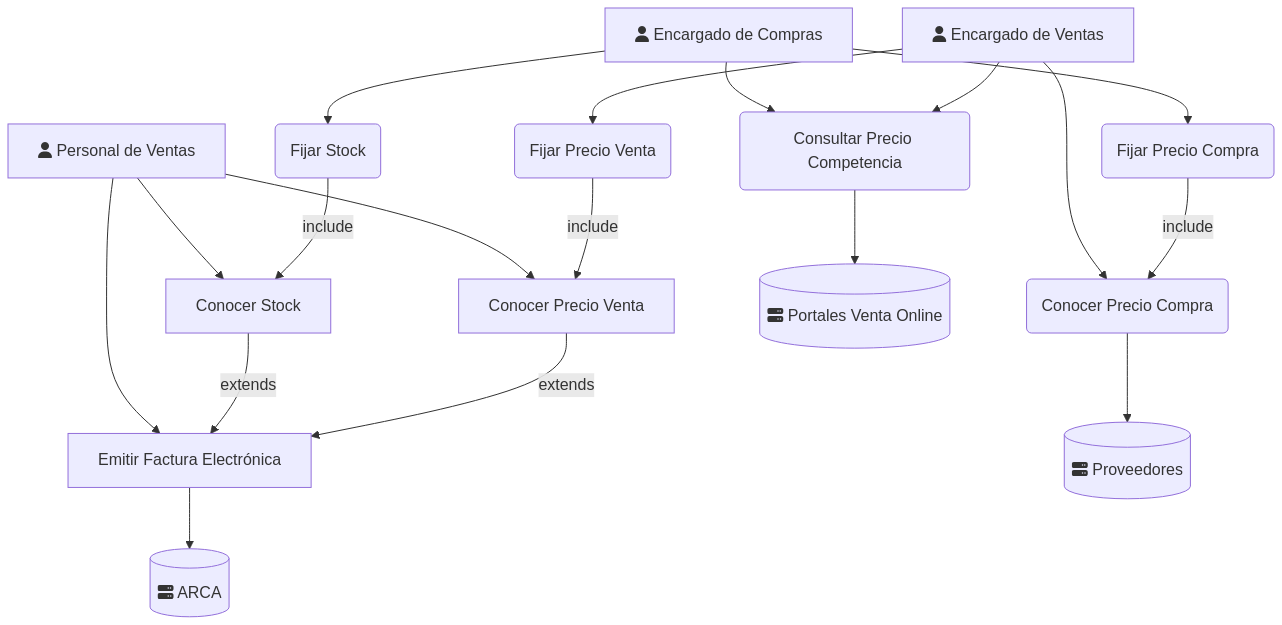
\includegraphics[width=\textwidth]{img/01-diagrama-casos-uso}
	\caption{Diagrama de casos de uso}
	\vspace{15pt}
\end{figure}

\pagebreak

\section{Descripción resumida de casos de uso}

\subsection{Consultar precios disponibles para un producto}

Dado un número de parte (nomenclador único de un producto),
el encargado de compras contará con un listado de precios de dicho producto,
que será descargado de las páginas web e interfaces de programación de los diversos proveedores,
según el caso.

\textbf{Actores:} Encargado de compras (primario), proveedores (secundario).

\subsection{Conocer los precios de la competencia}

Dado un número de parte,
el encargado de compras contará con un listado de precios de venta del producto,
que se descargará de páginas web y APIs de los portales de venta online,
de acuerdo a su disponibilidad.

\textbf{Actores:} Encargado de compras (primario), Portales de venta online de la competencia (secundario).

\subsection{Seguir el stock disponible, previendo necesidades de corto y mediano plazo.}

Dado un número de parte,
el encargado de compras debe contar con un número de stock disponible de un producto y,
de ser necesario,
actualizar el stock.

\textbf{Actores:} Encargado de compras (primario).

\subsection{Concretada una compra, fijar un precio de compra en el sistema}

Tomada una decisión de compra,
en base a la información disponible sumistrada por el sistema,
el encargado de compras fijará un precio de compra en el sistema,
que servirá como parámetro para el encargado de ventas.

\textbf{Actores:} Encargado de compras (primario).


\subsection{Conocer los precios de recompra para un producto}

El encargado de ventas puede necesitar la información del costo de recompra de un producto,
para reaccionar a un cambio en el precio de mercado.
En ocasiones, un precio de mercado de un producto puede caer,
y el encargado de ventas debe ser capaz de reaccionar a ello.
Este precio se tomará del fijado por el encargado de compras.

\textbf{Actores:} Encargado de ventas (primario).

\subsection{Conocer los precios de la competencia}

Para determinar un precio competitivo,
que cuide a los clientes al tiempo que asegura rentabilidad a la empresa,
el encargado de ventas debe de disponer del precio de mercado.
Para ello, 
dado un número de parte,
el encargado de ventas contará con un listado de precios,
obtenido de portales de venta de la competencia, 
como son Mercado Libre, Amazon y otros.
Con esta información, 
el encargado de ventas definirá los precios de lista de los productos,
que será el precio al consumidor final.

\textbf{Actores:} Encargado de ventas (primario), portales de venta online (secundario).

\subsection{Fijar precio para un producto}

Dado el precio de recompra y el precio de mercado,
el encargado de ventas fijará un precio a consumidor final de un producto,
procurando un equilibrio entre competitividad y rentabilidad de la empresa.
El precio de venta fijado para un producto será luego leído por el personal de ventas,
para la atención al público y la emisión de factura electrónica.

\textbf{Actores:} Encargado de ventas (primario).

\subsection{Consultar precio de un producto}

El personal de venta atiende al comprador minorista y debe consultar el último precio disponible,
fijado ya por el encargado de ventas.
Estos precios pueden variar con relativa velocidad,
tanto al alza por una escasez relativa,
como a la baja para reaccionar a la creciente competencia,
y el personal de ventas debe estar sincronizado con dichos cambios.

\textbf{Actores:} Personal de ventas (primario).

\subsection{Confirmar disponibilidad de stock de producto al consumidor final que lo requiera.}

En la atención al cliente minorista,
el personal de venta debe disponer de información relativa a los stocks,
para confirmar existencia de producto en depósito.

\textbf{Actores:} Personal de ventas (primario).

\subsection{Emitir factura electrónica}

El personal de ventas, 
luego de la brindar atención y asesoramiento al comprador minorista,
puede utiliza la información del sistema
-descripción del producto, cantidad, disponibilidad y precio-
para emitir una factura electrónica.
Esto puede hacerse sincronizando al sistema con la API de la ex AFIP,
ahora ARCA.
Por último,
concretada la venta,
el sistema debe imputar la reducción de stock correspondiente.

\textbf{Actores:} Personal de ventas (primario), Sistema de ARCA (secundario).
